\documentclass{article}

\usepackage{graphicx}
\usepackage{tikz}
\usepackage{tikzsymbols}
\usetikzlibrary{calc,patterns,shapes.geometric}
\pagestyle{empty}
\usepackage[margin=0pt]{geometry}
\geometry{papersize={14in,12in}}

\def\centerarc[#1](#2)(#3:#4:#5){\draw[#1] ($(#2)+({#5*cos(#3)},{#5*sin(#3)})$) arc (#3:#4:#5);}

\begin{document}
	\begin{figure}
		\centering
		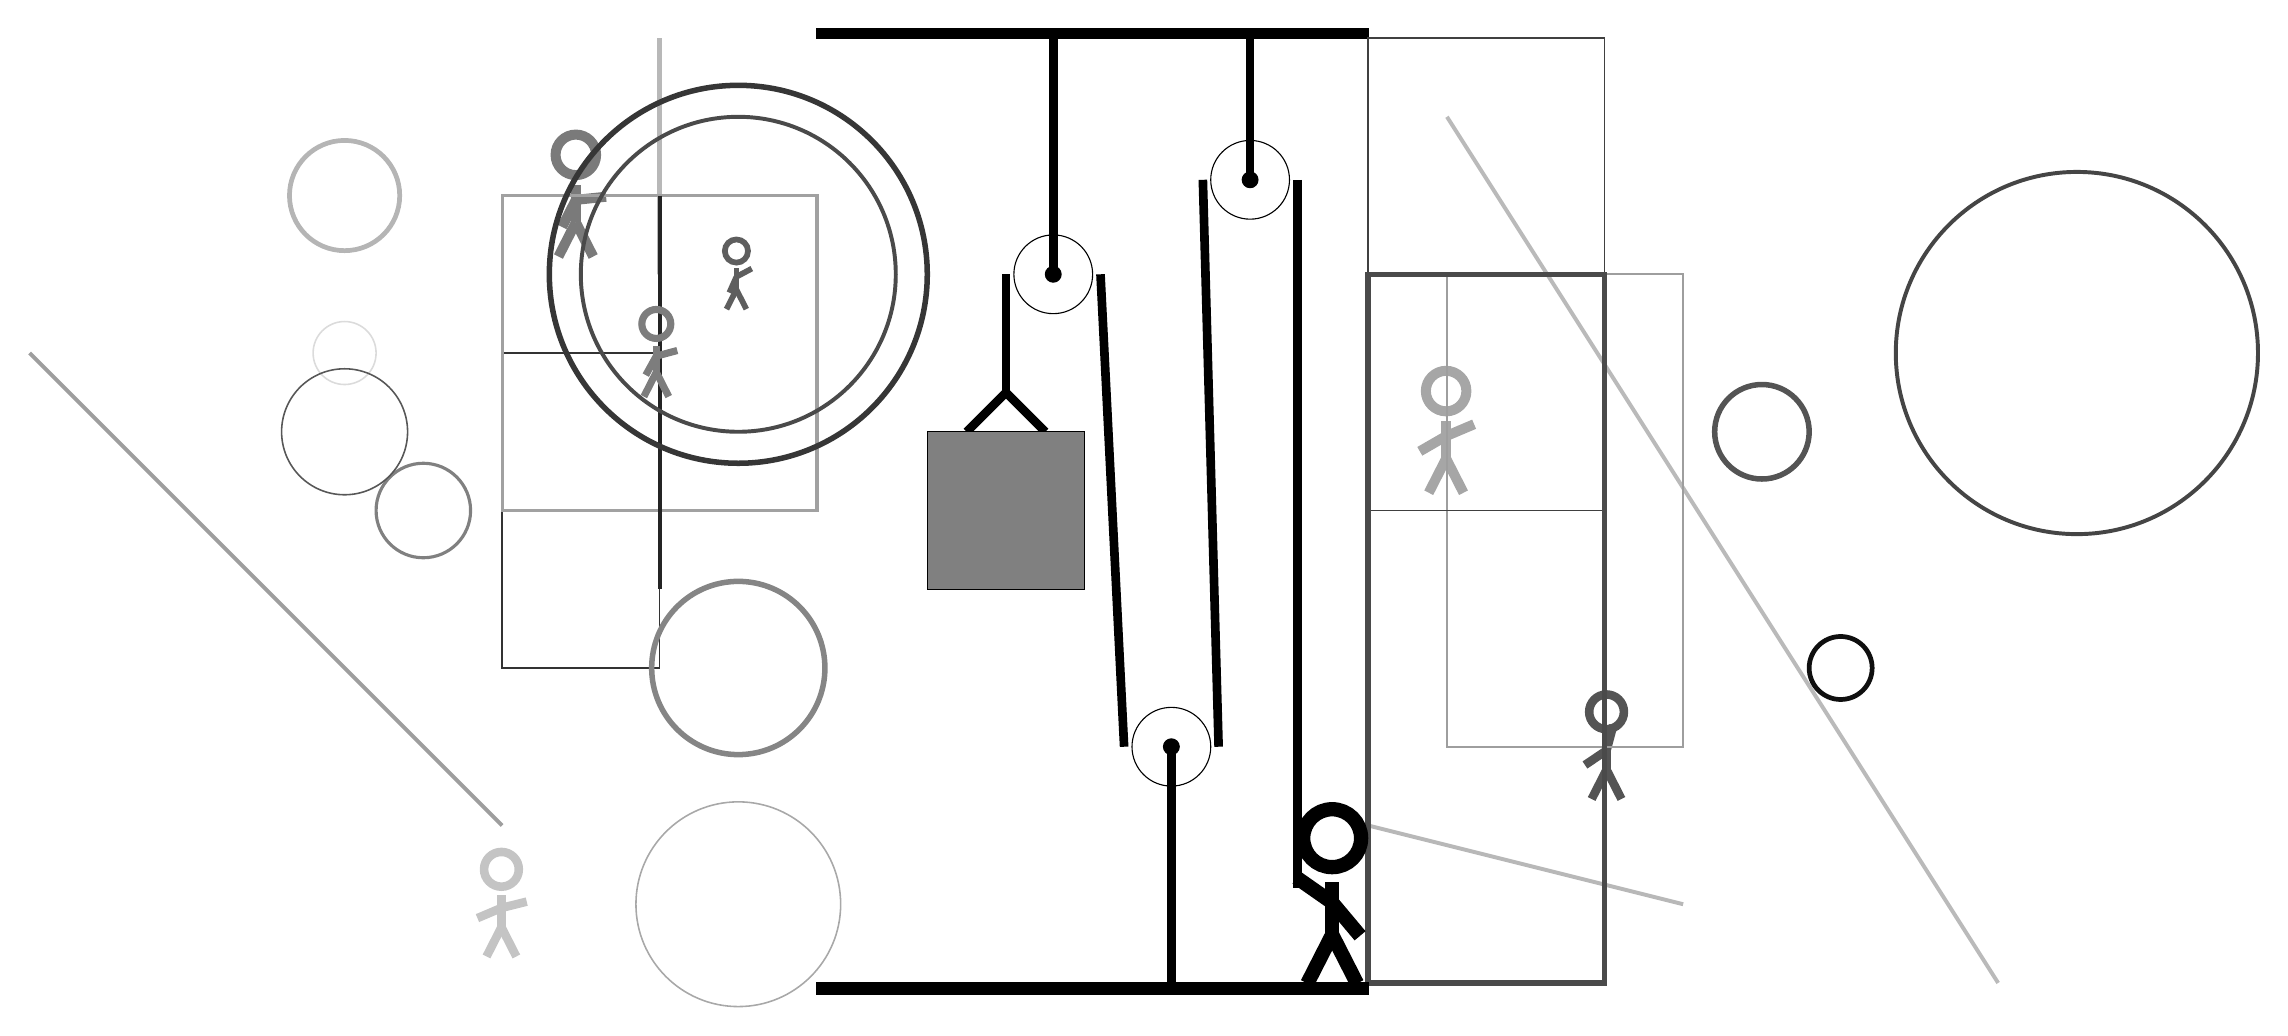
\begin{tikzpicture}
			%%%%% START %%%%%
			
			\draw[fill=black] (-2, 9) rectangle (5, 9.125);
			
			\draw [line width=0.6mm, color=black!63](-7, 1) circle (0.0);
			
			\node[line width=0.6mm, color=black!67] at (8, 0) {\Strichmaxerl[6][34][75]};
			\draw [line width=0.4mm, color=black!50](-7, 3) circle (0.6);
			\draw[line width=0.5mm, color=black!28](9, -2) -- (5, -1);
			\draw [line width=0.2mm, color=black!14](-8, 5) circle (0.4);
			\draw[line width=0.7mm, color=black!28] (-4, 6) rectangle (-4, 9);
			\draw[line width=0.2mm, color=black!80] (-4, 5) rectangle (-6, 1);
			
			\node[line width=0.6mm, color=black!35] at (6, 4) {\Strichmaxerl[7][30][23]};
			\draw [line width=0.5mm, color=black!73](14, 5) circle (2.3);
			
			\draw[line width=0.5mm, color=black!27](6, 8) -- (13, -3);
			\node[line width=0.3mm, color=black!63] at (-3, 6) {\Strichmaxerl[4][66][28]};
			\node[line width=0.3mm, color=black!52] at (-5, 7) {\Strichmaxerl[7][63][6]};
			\draw[line width=0.4mm, color=black!37] (-2, 3) rectangle (-6, 7);
			
			\draw [line width=0.2mm, color=black!66](-8, 4) circle (0.8);
			\draw [line width=0.6mm, color=black!94](11, 1) circle (0.4);
			\draw [line width=0.7mm, color=black!67](10, 4) circle (0.6);
			
			\draw[line width=0.2mm, color=black!38] (6, 0) rectangle (9, 6);
			
			\draw[line width=0.5mm, color=black!86](-4, 7) -- (-4, 2);
			\draw [line width=0.7mm, color=black!79](-3, 6) circle (2.4);
			
			\draw [line width=0.5mm, color=black!71](-3, 6) circle (2.0);
			\draw [line width=0.6mm, color=black!29](-8, 7) circle (0.7);
			
			\draw [line width=0.2mm, color=black!34](-3, -2) circle (1.3);
			
			\draw[line width=0.5mm, color=black!38](-6, -1) -- (-12, 5);
			\node[line width=0.3mm, color=black!51] at (-4, 5) {\Strichmaxerl[5][61][15]};
			\draw[line width=0.2mm, color=black!75] (5, 9) rectangle (8, 3);
			
			\node[line width=0.5mm, color=black!23] at (-6, -2) {\Strichmaxerl[6][23][14]};
			\draw [line width=0.7mm, color=black!48](-3, 1) circle (1.1);
			\draw[line width=0.7mm, color=black!71] (5, 6) rectangle (8, -3);
			
			\draw (1, 6) circle (0.5);
			\draw[fill=black] (1, 6) circle (0.1);
			\draw[line width=1.1mm]  (1, 9) -- (1, 6);
			
			\draw[fill=white](2.5, 0) circle (0.5);
			\draw[fill=black] (2.5, 0) circle (0.1);
			\draw[line width=1.1mm]  (2.5, -3) -- (2.5, 0);
			
			\draw[fill=white](3.5, 7.2) circle (0.5);
			\draw[fill=black] (3.5, 7.2) circle (0.1);
			\draw[line width=1.1mm] (3.5, 9) -- (3.5, 7.2);
			
			\draw[line width=1.1mm] (-0.1, 4.0) -- (0.4, 4.5) -- (0.9, 4.0);
			\draw[fill=black!50] (-0.6, 4.0) rectangle (1.4, 2.0);
			
			\draw[line width=1.1mm] (0.4, 6) -- (0.4, 4.5);
			\centerarc[line width=1.1mm](1, 6)(0:180:0.6);
			\draw[line width=1.1mm](1.6, 6) -- (1.9, 0);
			\centerarc[line width=1.1mm](2.5, 0)(180:360:0.6);
			\draw[line width=1.1mm](3.1, 0) -- (2.9, 7.2);
			\centerarc[line width=1.1mm](3.5, 7.2)(0:180:0.6);
			\draw[line width=1.1mm](4.1, 7.2) -- (4.1, -1.8);
			
			\node at (4.5, -1.9) {\Strichmaxerl[10][-35][-50]};
			
			\draw[fill=black] (-2, -3) rectangle (5, -3.15);
			
			%%%%% END %%%%%
		\end{tikzpicture}
	\end{figure}	
\end{document}